\chapter{Stochastic Switching Linear Control using Linear Hybrid Models}
\label{sec_rbpf_control}
In Section \ref{sec_switch_mpc_lit} model switching MPC was discussed. In short, a set of models with corresponding binary integer variables are incorporated into the MPC optimisation problem. The optimisation algorithm changes the model it uses for prediction based on the location of the previous predicted state. In this way a number of models can potentially be used for prediction. It is desirable to change models if the system states move far away from the linearisation point of current linear model. It is hoped that the significant computational burden this introduces is offset by the increased predictive accuracy of the controller.

In Section \ref{sec_linear_control} we developed an efficient stochastic MPC algorithm which uses a single linear model for control. While it is possible to attempt to extend that algorithm to the aforementioned approach, the computational problems will persist because Mixed Integer Programming is fundamentally more difficult than Quadratic Programming \cite{forst}. From a practical perspective one would like to reduce computational complexity because, especially for large problems, on-line optimisation can become problematic.

In Section \ref{sec_inf_lin_hybrid} the Rao-Blackwellised Particle Filter was introduced. Briefly, the filter uses a set of linear models, $M_i=(A_i, B_i)$ for each model $i$, to estimate the current state (we assume the system and measurement noise is common across all models as well as the observation matrix). The ability of each model to explain the observations is calculated in a Bayesian sense. This is used to weight the importance of each model's contribution to the current state estimate. 

In this section we will attempt to combine the ideas of Section \ref{sec_switch_mpc_lit}, \ref{sec_linear_control} and \ref{sec_inf_lin_hybrid} to create a computationally efficient switching model MPC algorithm. We first describe the intuition behind the approach and then state the algorithm.

As mentioned before, it becomes desirable to have a mechanism to switch the underlying controller model if the system states move far away from the linearisation point of the current model. However, it is computationally difficult to perform this switching within the framework of the optimisation algorithm because it invariably necessitates the introduction of integer variables. We propose an algorithm which uses the RBPF to estimate the current state as well as the model which best describes the observations. Based on the results of Section \ref{sec_inf_lin_hybrid} we expect this model to be the one closest to the current state. This most likely model is then used within the framework of the predictive control introduced in Section \ref{sec_linear_control}. Thus the controller uses a single linear model for control but this model can be switched depending on the current position of the system states in state space. The algorithm is shown below:

\textbf{Switching Controller Algorithm}:
\begin{enumerate}
\item
Use a switching filter algorithm, e.g. the RBPF, to update the state estimates of the particle population given the current observation. See Section \ref{sec_inf_lin_hybrid} for more details.
\item
Select the particle with the highest switching weight. Since each particle corresponds to a certain model we implicitly have the most probable model $M_i$.
\item
Use the mean and covariance information encoded by this particle within the context of the stochastic controller (LQG and MPC) formulation of Section \ref{sec_linear_control}. Use the most likely model, $M_i$ from step 2, in this setting.
\item
Repeat for the next observation. 
\end{enumerate} 
The astute reader will notice that we are implicitly using the Graphical Model shown in Figure \ref{fig_gm_filter} for state estimation (filtering) but the Graphical Model of Figure \ref{fig_gm_prediction} for model based prediction in step 3.
\begin{figure}[H] 
\centering
\begin{tikzpicture}

  % Define nodes
  \node[obs] (ya) {$y_{0}$};
  \node[obs, right=of ya] (yb) {${\hdots}$};
  \node[obs, right=of yb] (yc) {$y_{t}$};
  \node[latent, above=of ya]  (xa) {$x_{0}$};
  \node[latent, above=of yb, right=of xa]  (xb) {${\hdots}$};
  \node[latent, above=of yc, right=of xb]  (xc) {$x_{t}$};
  \node[det, above=of xa, xshift=0.7cm] (da) {$u_{0}$};
  \node[det, above=of xb, xshift=0.7cm] (db) {$u_{t-1}$};
  \node[latent, above=of xa, yshift=1.1cm] (sa) {$s_{0}$};
  \node[latent, above=of xb, yshift=1.1cm] (sb) {${\hdots}$};
  \node[latent, above=of xc, yshift=1.1cm] (sc) {$s_{t}$};
  
  % Connect the nodes
  \edge {da} {xb};
  \edge {db} {xc};
  \edge {xa} {ya};
  \edge {xb} {yb};
  \edge {xc} {yc};
  \edge {xa} {xb};
  \edge {xb} {xc};
  \edge {sa} {sb};
  \edge {sb} {sc};
  \edge {sa} {xa};
  \edge {sb} {xb};
  \edge {sc} {xc};
  
\end{tikzpicture}
\caption{Graphical Model used for state estimation.}
\label{fig_gm_filter}
\end{figure}
\begin{figure}[H] 
\centering
\begin{tikzpicture}

  % Define nodes
  \node[obs] (ya) {$y_0$};
  \node[latent, above=of ya]  (xa) {$x_0$};
  \node[latent, above=of yb, right=of xa]  (xb) {$x_1$};
  \node[latent, above=of yc, right=of xb]  (xc) {$x_2$};
  \node[det, above=of xa, xshift=0.7cm] (da) {$u_0$};
  \node[det, above=of xb, xshift=0.7cm] (db) {$u_1$};
  \node[latent, above=of xa, yshift=1.1cm] (sa) {$s_0$};
  
  % Connect the nodes
  \edge {da} {xb};
  \edge {db} {xc};
  \edge {xa} {ya};
  \edge {xa} {xb};
  \edge {xb} {xc};
  \edge {sa} {xa};
\end{tikzpicture}
\caption{Simplified Graphical Model used for prediction. Within the context of MPC prediction we have that $x_t=x_0$ at each successive time step.}
\label{fig_gm_prediction}
\end{figure}
We are not using the Graphical Model associated with Rao-Blackwellised Particle Prediction (see Section \ref{sec_inf_rbpf_pred}) because that would require that we incorporate stochastic model switching within the optimisation algorithm. 

For the remainder of this section we assume that we have a bank of $M=3$ linear models and that we measure both states. Each model is derived by linearising the non-linear CSTR model, found in Section \ref{sec_cstr}, around the nominal operating points discussed in the same section as well as Section \ref{sec_rbpf_filtering_cstr}. We also use the switching transition matrix $P_2$ found in (\ref{eq_switch_trans}).
\section{Unconstrained Switching Control}
\label{sec_rbpf_control_uncon}
Due to the analysis of Section \ref{sec_uncon_lin_control} we know that is is possible to convert the stochastic optimisation problem (\ref{eq_rbpf_lqg}) into the deterministic optimisation problem (\ref{eq_rbpf_lqr}) for each linear model $(M_1, M_2, M_3)$ given that we have the state estimate of the initial value $x_0$, the dynamics are linear and the underlying distributions are Gaussian. Throughout this section we make these assumptions. As before, we also denote the mean and covariance of the current state estimate $x_0$ by $\mathbb{E}[x_0]=\mu_0$ and $\text{var}[x_0]=\Sigma_0$.
\begin{equation}
\begin{aligned}
&\underset{\mathbf{u}}{\text{min }} \mathbb{E}\left[ \frac{1}{2}\sum_{k=0}^{N-1} \left( x_k^TQx_k + u_k^TRu_k \right) + \frac{1}{2}x_N^TP_fx_N \right] \\
& \text{subject to } x_{t+1}=A_ix_t+B_iu_t + w_t~\text{(Latent)} \\
& \text{and } y_{t}= Cx_t + v_t \text{ (Observed)}\\
\end{aligned}
\label{eq_rbpf_lqg}
\end{equation}
We have that (\ref{eq_rbpf_lqg}) is equivalent to (\ref{eq_rbpf_lqr}) under the aforementioned assumptions.
\begin{equation}
\begin{aligned}
&\underset{\mathbf{u}}{\text{min }} \frac{1}{2}\sum_{k=0}^{N-1} \left( \mu_k^TQ\mu_k + u_k^TRu_k \right) + \frac{1}{2}\mu_N^TP_f\mu_N + \frac{1}{2}\sum_{k=0}^N \text{tr}(Q\Sigma_k) \\
&\text{with } \mu_{t+1} = A_i\mu_t +B_iu_t \\
&\text{and } \Sigma_{t+1} = W+A_i\Sigma_t A_i^T 
\end{aligned}
\label{eq_rbpf_lqr}
\end{equation}
Given this we apply the Switching Controller Algorithm within the context of the LQG controller i.e. given a model we solve the LQG problem and implement that input. In light of our analysis in Section \ref{sec_linear_control} it is clear that the Switching Controller Algorithm is straightforward to implement because it simplifies to the deterministic LQR controller. We assume the underlying plant is non-linear with state and observation noise as well as the controller parameters the same as those found in Section \ref{sec_lin_sys_cont}.

As mentioned before we only use the most likely model for control purposes. By only selecting one to use for control we dramatically simplify the control problem. It allows us to use the controllers of Section \ref{sec_linear_control} directly. We study two control problems using the Switching Controller Algorithm in this section. The first problem is to drive the non-linear CSTR to the low temperature operating point i.e. the concentration set point is $0.998~\text{kmol.m}^{-3}$. The second problem is to drive the non-linear CSTR to a concentration set point of $0.95~\text{kmol.m}^{-3}$. On both cases we use the LQG controller as shown in (\ref{eq_rbpf_lqg}).

We investigate the first problem in Figures \ref{fig_rbpf_control_state} to \ref{fig_rbpf_control_track}. In Figure \ref{fig_rbpf_control_state} we see the state space trajectory of the system under control. We expect $M_2$ to be active initially after which only $M_3$ should be active.
\begin{figure}[H] 
\centering
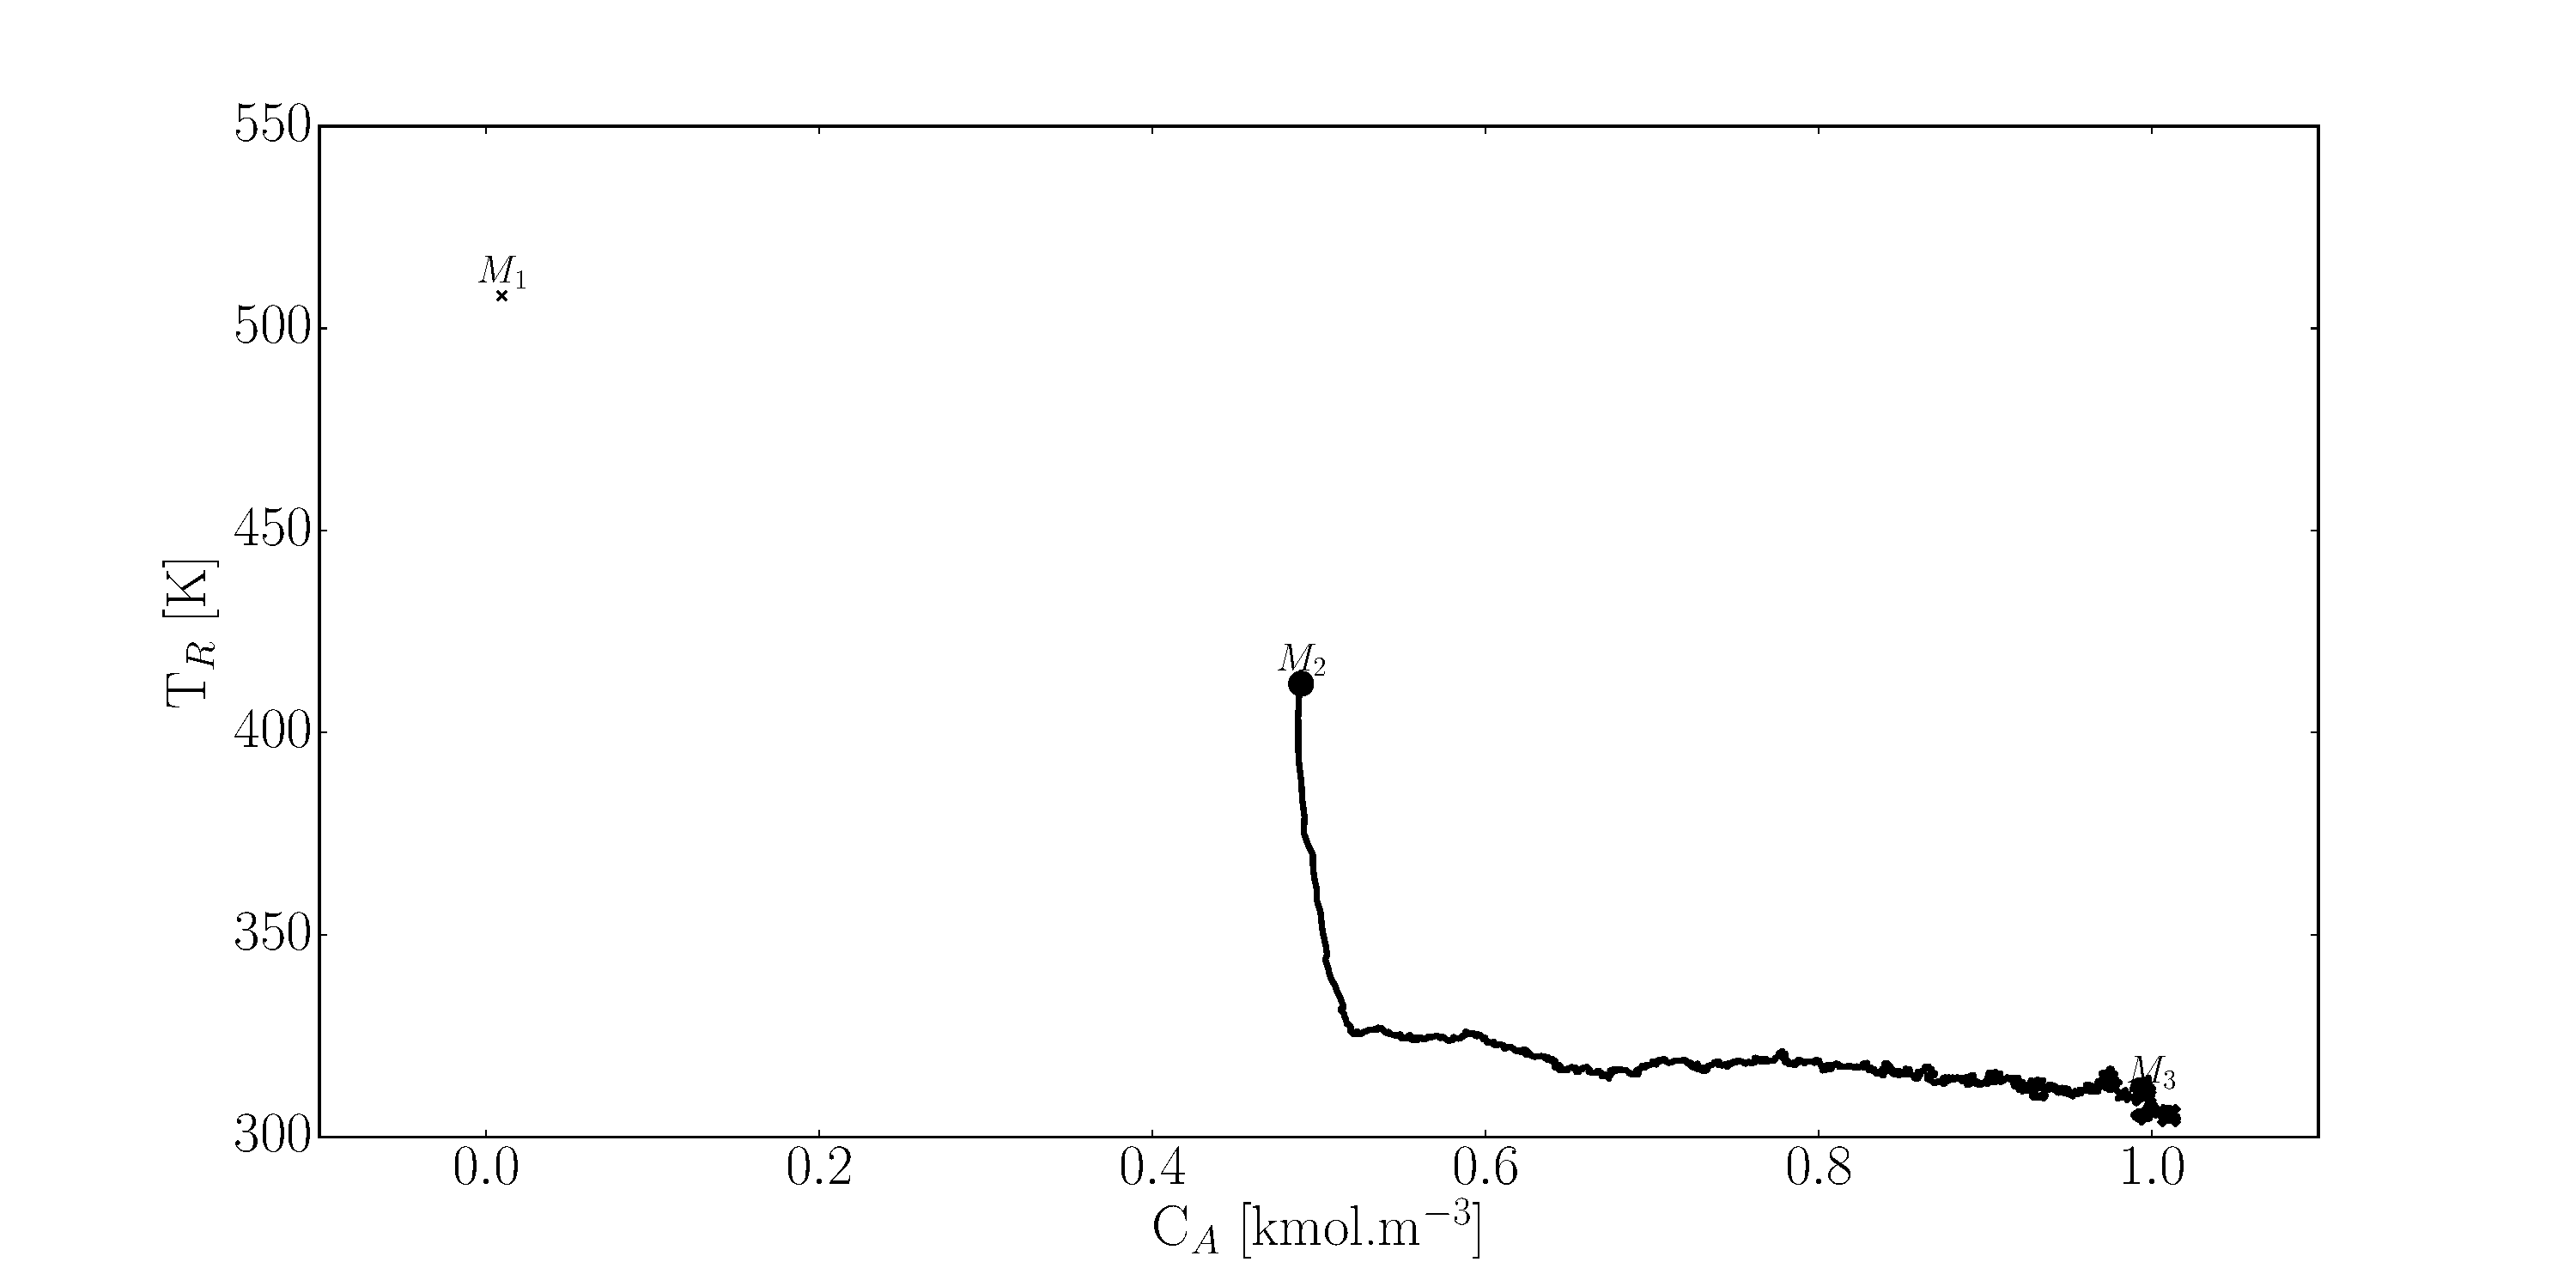
\includegraphics[scale=0.25]{rbpf_control_state.pdf}
\caption{State space trajectory of the non-linear CSTR under control of the LQG Switching Controller Algorithm. The initial point was $(0.5, 400)$}
\label{fig_rbpf_control_state}
\end{figure}
In Figure \ref{fig_rbpf_control_switch} we see that initially $M_2$ best explained the observations but that $M_3$ was predominantly used throughout the rest of the simulation.   
\begin{figure}[H] 
\centering
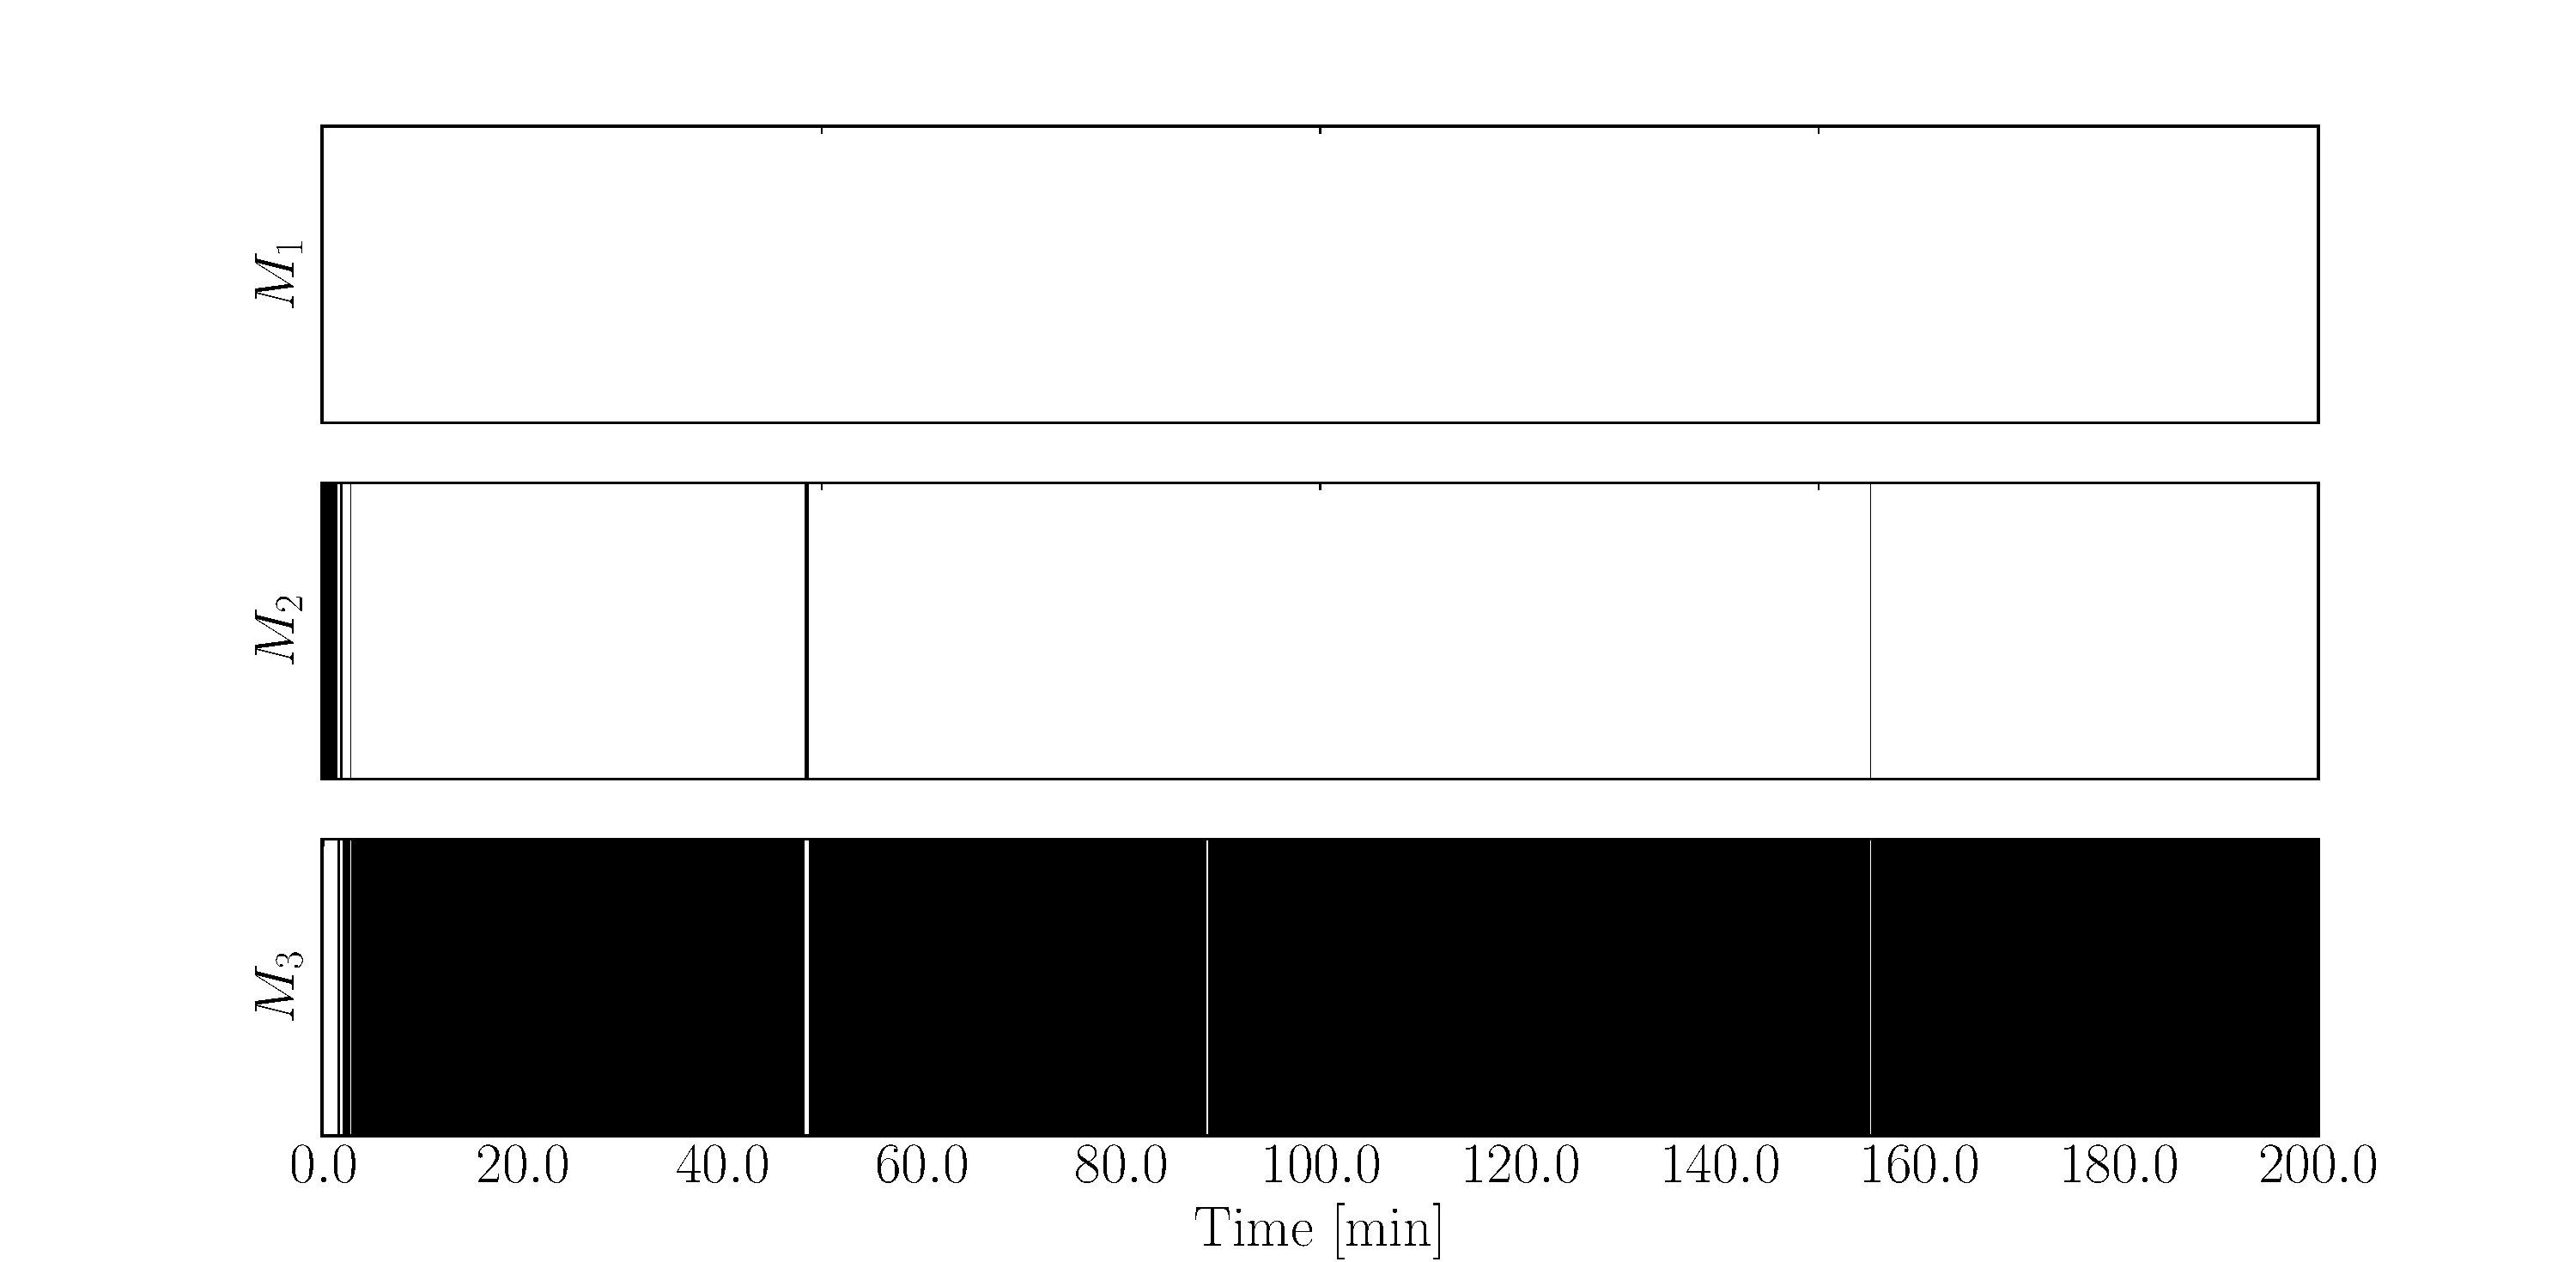
\includegraphics[scale=0.25]{rbpf_control_switch.pdf}
\caption{Most likely model used for control at each time step over the simulation. Black indicates the model was not used.}
\label{fig_rbpf_control_switch}
\end{figure}
However, it is clear that there are some problems in Figure \ref{fig_rbpf_control_switch}. There does seem to be some switching noise - especially near the end of the simulation where we do not expect $M_2$ to be present at all. Given that we are using the sticky switching transition matrix $P_2$ it is clear that model overlap is again causing problems. The same problem was identified in Section \ref{sec_rbpf_filtering_cstr}.

In Figure \ref{fig_rbpf_control_track} we see the consequence of the switching noise.
\begin{figure}[H] 
\centering
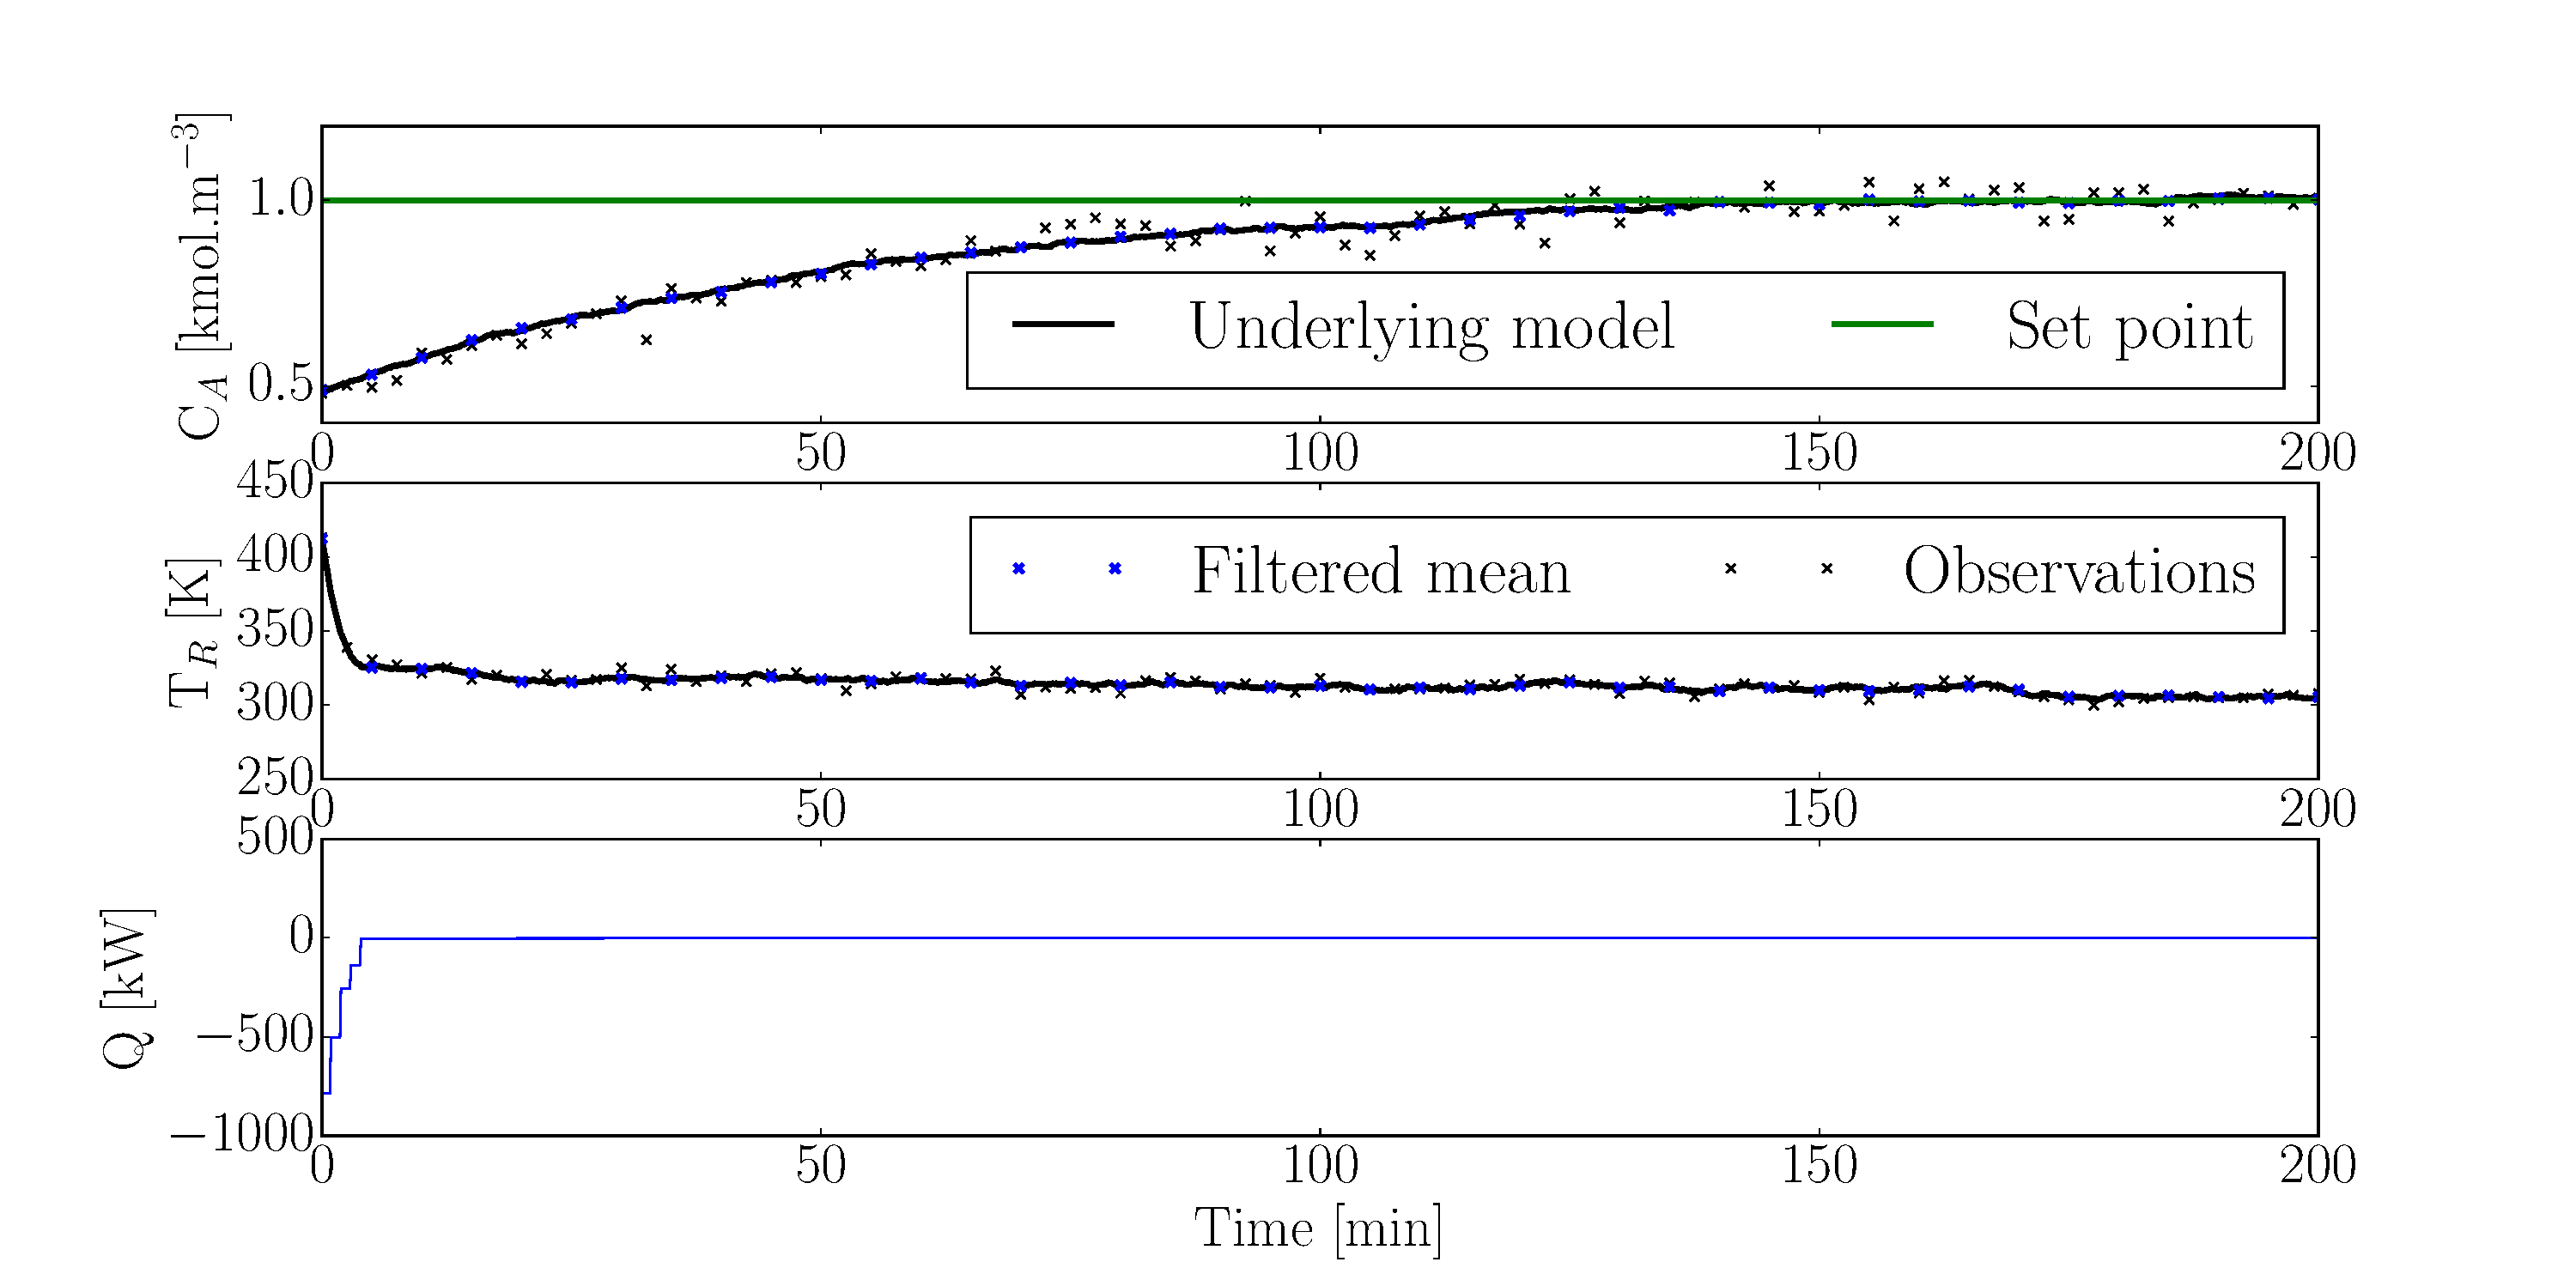
\includegraphics[scale=0.25]{rbpf_control_track.pdf}
\caption{Set point tracking and controller input for the LQG Switching Controller Algorithm. The initial point was $(0.5, 400)$.}
\label{fig_rbpf_control_track}
\end{figure}
Although the controller manages to track the set point we see spikes in controller input occurring whenever the model is switched. While we expect this initially - when the system moves from the regime of $M_2$ to the regime of $M_3$, it is unexpected later. Clearly switching noise is potentially bad for control.

In Figures \ref{fig_rbpf_control_switch2} and \ref{fig_rbpf_control_track2} we study problem 2: the concentration set point is $0.95~\text{kmol.m}^{-3}$. In Figure \ref{fig_rbpf_control_switch2} we see even more switching noise than before.
\begin{figure}[H] 
\centering
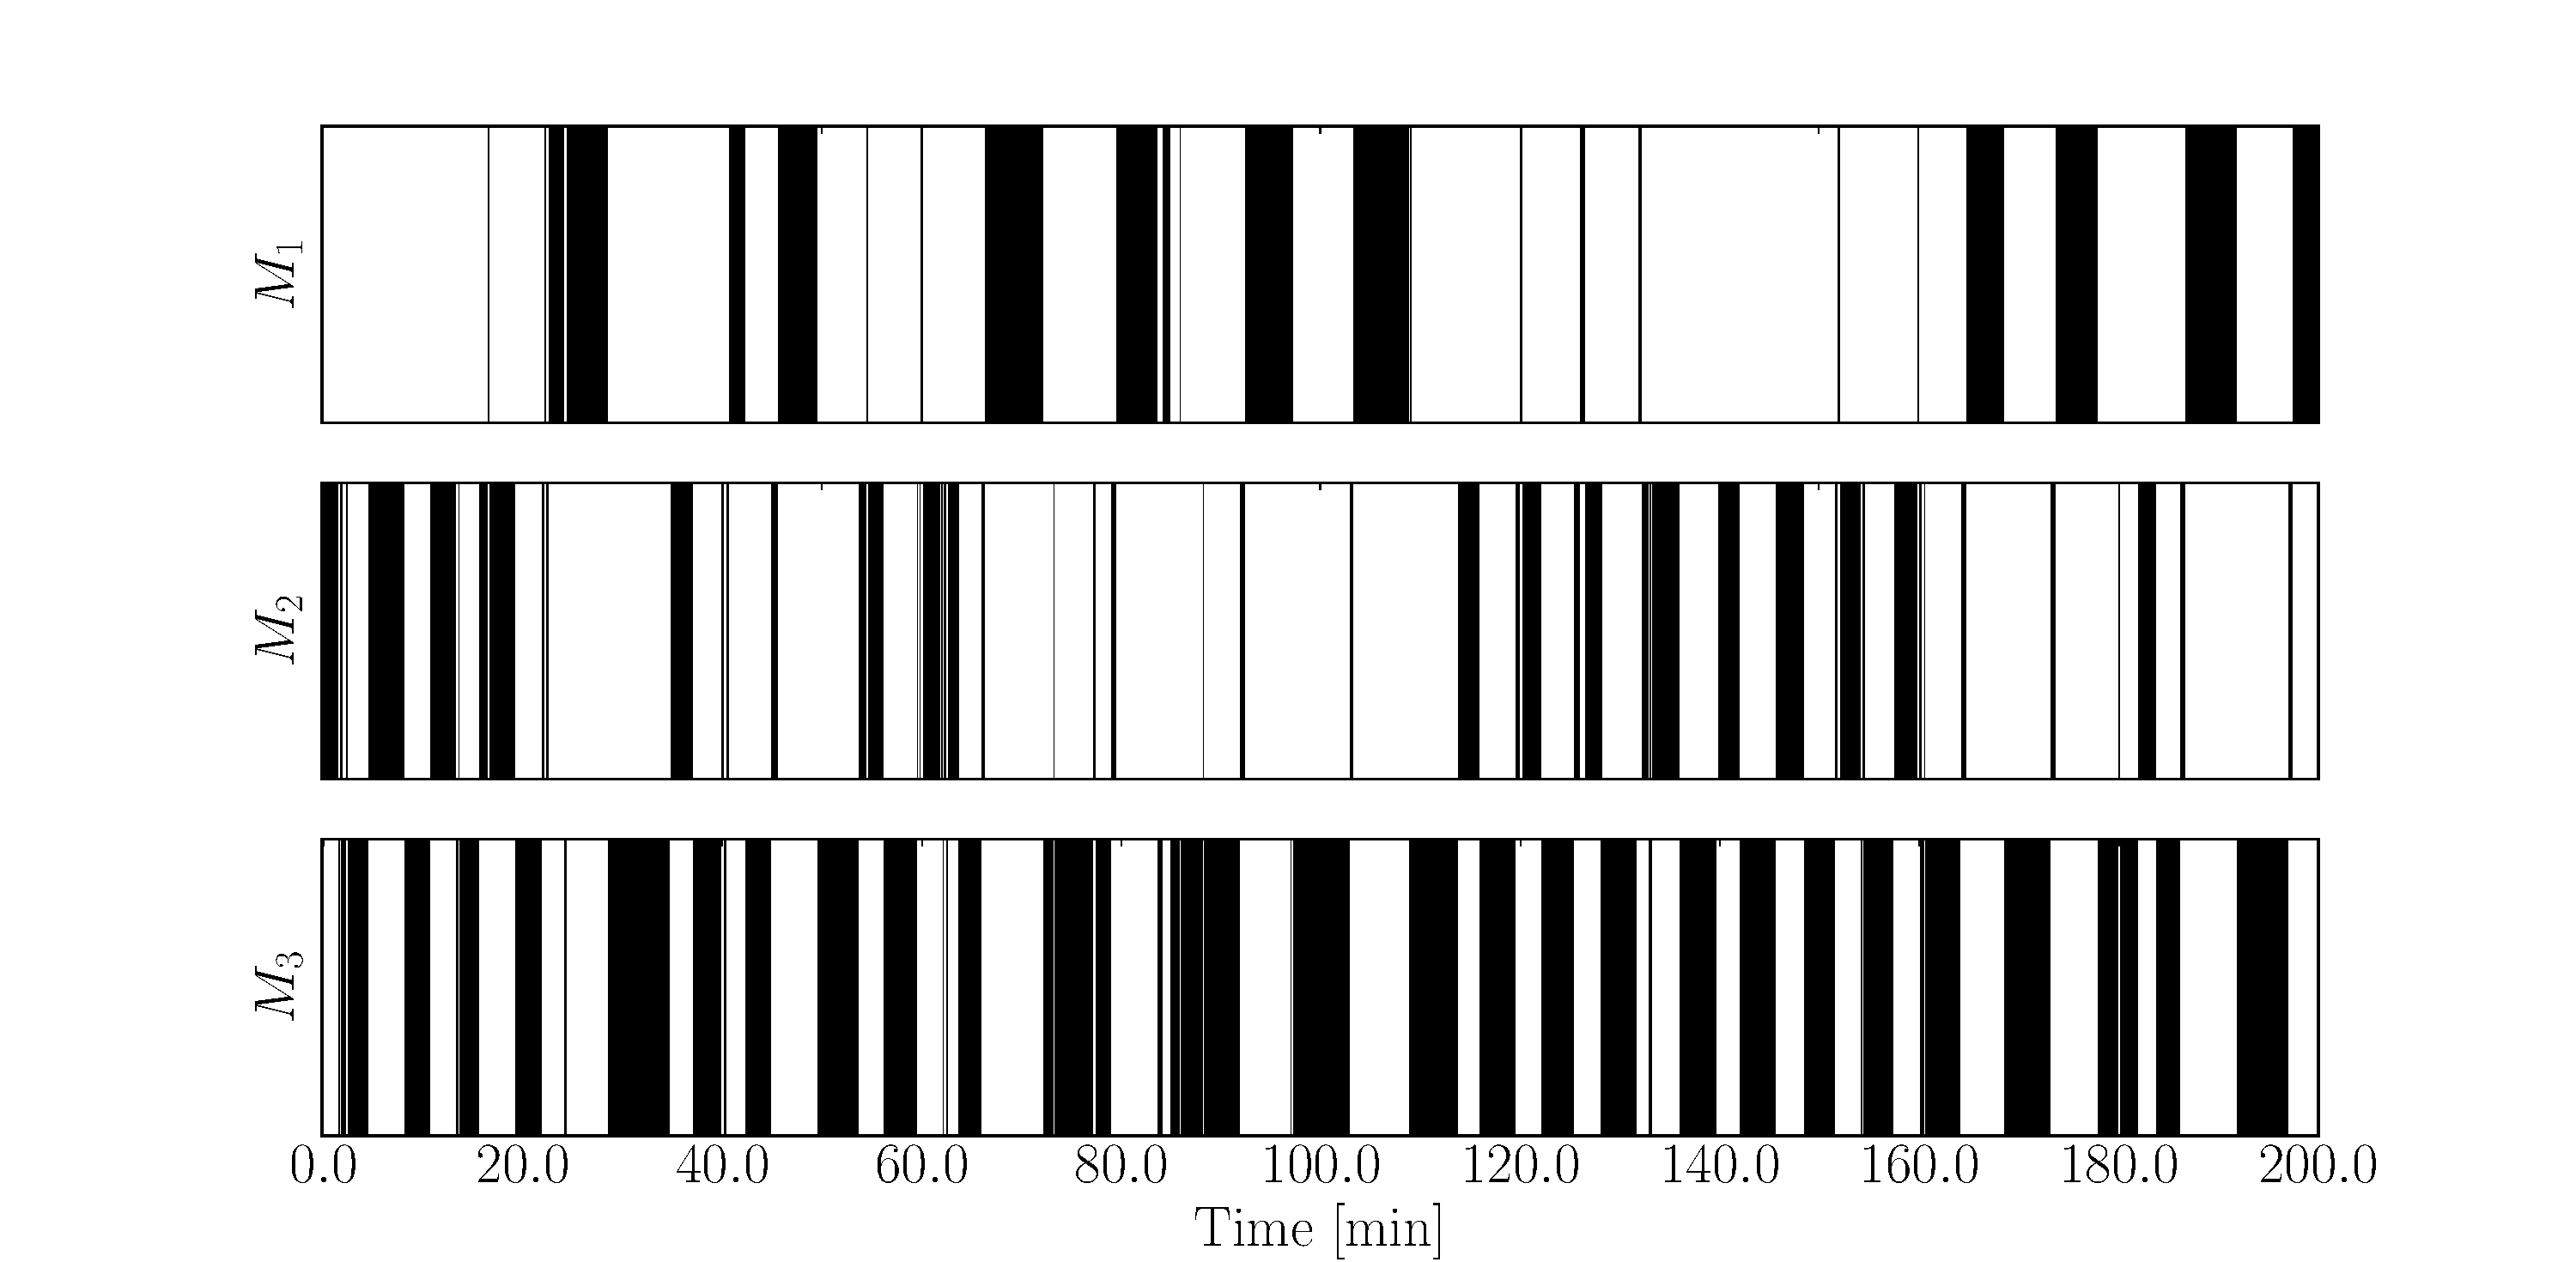
\includegraphics[scale=0.25]{rbpf_control_switch2.pdf}
\caption{Most likely model used for control at each time step over the simulation. Black indicates the model was not used.}
\label{fig_rbpf_control_switch2}
\end{figure}
In Figure \ref{fig_rbpf_control_track2} the detrimental consequence of the switching noise is evident. The controller is completely unstable and oscillates.
\begin{figure}[H] 
\centering
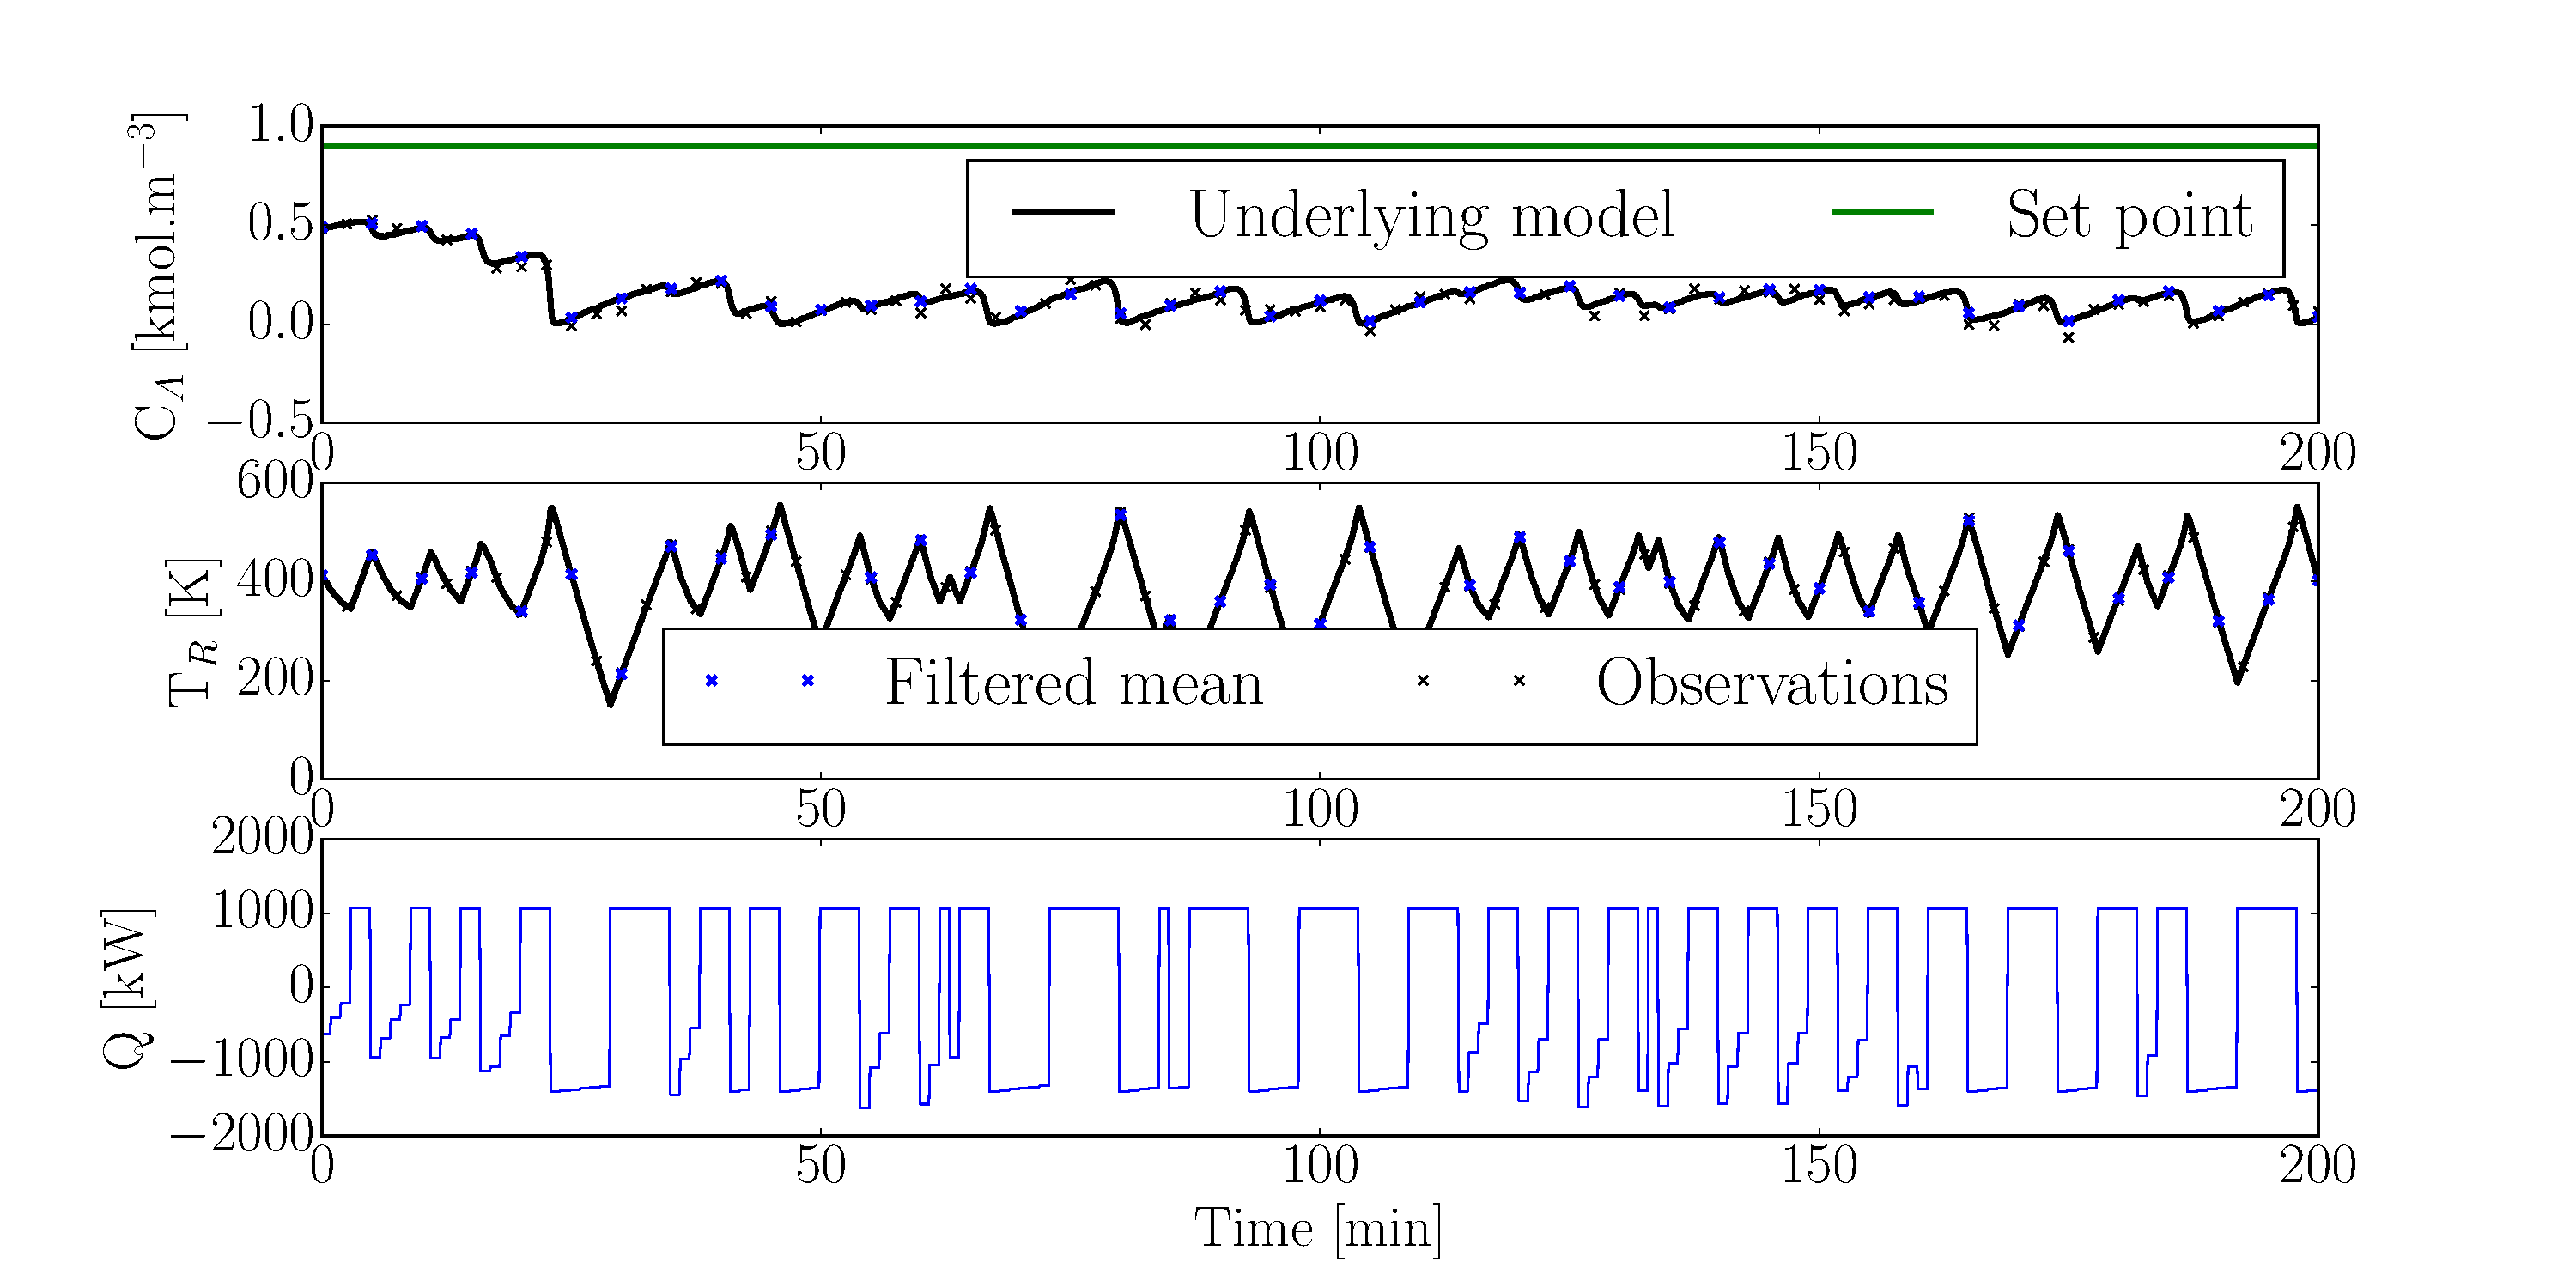
\includegraphics[scale=0.25]{rbpf_control_track2.pdf}
\caption{Set point tracking and controller input for the LQG Switching Controller Algorithm. The initial point was $(0.5, 400)$.}
\label{fig_rbpf_control_track2}
\end{figure}
It is clear that the oscillations are caused by the filter's inability to stick to a model. While it is reasonable to surmise that the noise can be attenuated by making the switch transition matrix sticker, as we did in Section \ref{sec_rbpf_filtering_cstr}, the underlying problem will persist: the models are too similar for the switching filter to adequately differentiate between. Under these circumstances the inferred most probable model will likely always be noisy. The Switching Controller Algorithm, within the context of the RBPF, will not be a good controller until a method is found which properly addresses this issue.

The instability seen in Figure \ref{fig_rbpf_control_track2} arises because the current state has no effect on the switching transition matrix. Thus the probability of $M_3$ switching to $M_2$ does not change even if the current state is very close to the linearisation point of $M_3$. Clearly this is unrealistic. It should be investigated whether a more complex Graphical Model can fix this problem. The Graphical Model for the Augmented Switching Kalman Filter \cite{barber} is shown in Figure \ref{fig_gm_augmented}. 
\begin{figure}[H] 
\centering
\begin{tikzpicture}

  % Define nodes
  \node[obs] (ya) {$y_{0}$};
  \node[obs, right=of ya] (yb) {$y_{1}$};
  \node[obs, right=of yb] (yc) {$y_{2}$};
  \node[latent, above=of ya]  (xa) {$x_{0}$};
  \node[latent, above=of yb, right=of xa]  (xb) {$x_{1}$};
  \node[latent, above=of yc, right=of xb]  (xc) {$x_{2}$};
  \node[det, above=of xa, xshift=0.7cm] (da) {$u_{0}$};
  \node[det, above=of xb, xshift=0.7cm] (db) {$u_{1}$};
  \node[latent, above=of xa, yshift=1.1cm] (sa) {$s_{0}$};
  \node[latent, above=of xb, yshift=1.1cm] (sb) {$s_{1}$};
  \node[latent, above=of xc, yshift=1.1cm] (sc) {$s_{2}$};
  
  % Connect the nodes
  \edge {da} {xb};
  \edge {db} {xc};
  \edge {xa} {ya};
  \edge {xb} {yb};
  \edge {xc} {yc};
  \edge {xa} {xb};
  \edge {xb} {xc};
  \edge {sa} {sb};
  \edge {sb} {sc};
  \edge {sa} {xa};
  \edge {sb} {xb};
  \edge {sc} {xc};
  \edge {xa} {sb};
  \edge {xb} {sc};
    
\end{tikzpicture}
\caption{Augmented Switching Kalman Filter Graphical Model.}
\label{fig_gm_augmented}
\end{figure}
Using this model it is possible to specify the effect the state variables $(x_0,x_1,...)$ have on the switching variables $(s_0, s_1,...)$.  

\section{Conclusion}
In this section we introduced a controller which infers which \textit{model} predictive control should be based upon using a Rao-Blackwellised Particle Filter based upon the Switching Kalman Filter Graphical Model. Only the LQG controller was implemented using this scheme. It was found that the filter did not isolate the correct model robustly enough. For the control scheme to be effective the filter must not haphazardly switch between models. It was suggested that the current Graphical Model be extended to the Augmented Switching Kalman Filter Model because it potentially can address this issue.
